\documentclass{beamer}
\usepackage{graphicx}
\usepackage[most]{tcolorbox}
\usepackage{xcolor}
\definecolor{lightblue}{RGB}{25, 25, 112} % RGB-Werte für Hellblau

\usetheme{CambridgeUS} % Beispielhaftes ansprechendes Design

\usecolortheme{dolphin}

\title{Verteilte Systeme}
\subtitle{Einleitung und Abgrenzung}
\author{Prof. Dr. Martin Becke}
\date{\today}

\begin{document}

\begin{frame}
    \titlepage
\end{frame}

\begin{frame}{Verteilte Systeme in Hamburg}
    Hamburg, als bedeutender Wirtschaftsstandort, beherbergt zahlreiche Unternehmen, die auf innovative Technologien angewiesen sind. Verteilte Systeme spielen hier eine Schlüsselrolle, insbesondere in Branchen wie:

    \begin{itemize}
        \item \textbf{Hafenlogistik:} Der Hamburger Hafen als Smart Port nutzt verteilte Systeme für effizientes Ressourcenmanagement, Echtzeit-Datenanalyse und Automatisierung. Stellen Sie sich den Hafen wie ein komplexes Uhrwerk vor, dessen Zahnräder perfekt ineinandergreifen müssen – jedes Zahnrad ein Knoten im verteilten System.
        \item \textbf{Luftfahrt:} Airbus nutzt verteilte Systeme für sichere und effiziente Flugzeugsysteme.  Von Navigation bis zur Flugüberwachung kommunizieren verschiedene Komponenten in Echtzeit, ähnlich einem Orchester, das ein komplexes Musikstück spielt.
        \item \textbf{Finanzwesen:} Banken und Versicherungen nutzen verteilte Systeme für Echtzeit-Transaktionen und Datenverarbeitung. Stellen Sie sich ein Netzwerk von Bankautomaten vor: jeder Automat ein Knoten, der unabhängig arbeitet, aber Teil eines größeren, synchronisierten Systems ist.
    \end{itemize}

\end{frame}


\begin{frame}{Definition Verteilte Systeme}

    \begin{columns}[c] % Zentriert die Spalten

        \begin{column}{0.9\textwidth}
            \begin{figure}
                \centering
                \begin{tcolorbox}[colback=lightblue,arc=0pt,outer arc=0pt,boxrule=0pt,toprule=0pt,bottomrule=0pt,rightrule=0pt,leftrule=0pt] % Hellblauer Hintergrund, keine Rahmen
                    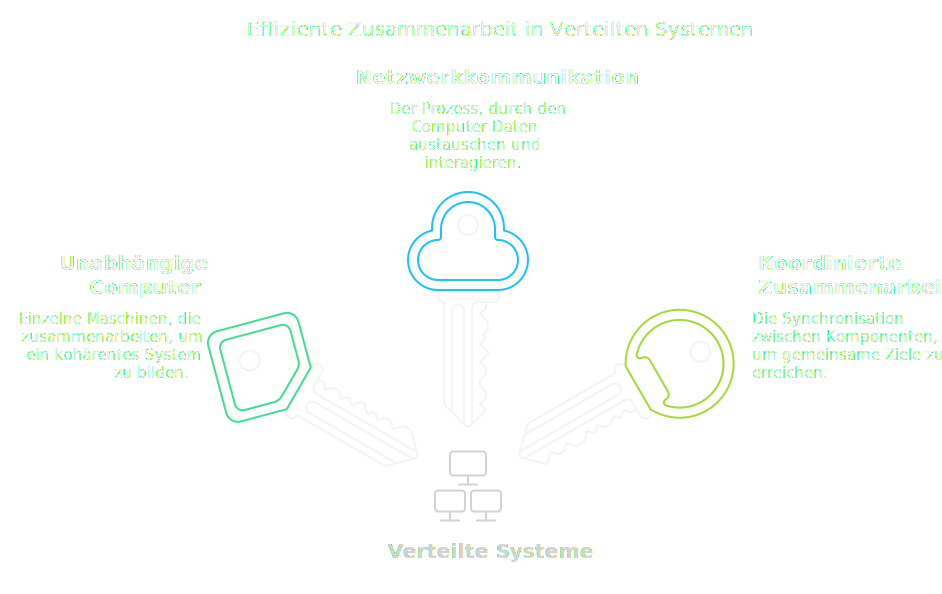
\includegraphics[width=1.0\textwidth]{fig/Definition-VS.png}
                \end{tcolorbox}
                \caption{Symbolbild Definition}
            \end{figure}
        \end{column}

        \note{ \textbf{Kerneigenschaft:} Kein gemeinsamer Speicher.  Die Kommunikation erfolgt über das Netzwerk, was Herausforderungen bei der Koordination mit sich bringt. }
    \end{columns}

\end{frame}

\begin{frame}{Definition Verteilte Systeme}

    \begin{columns}[c] % Zentriert die Spalten

        \begin{column}{1.0\textwidth} % Linke Spalte für den Text
            \begin{block}{Was sind verteilte Systeme?}
                \textbf{Tanenbaum:} Verteilte Systeme sind eine Gruppe von vernetzten, autonomen Computern, die für den Benutzer als ein kohärentes System erscheinen. Sie arbeiten zusammen, um eine gemeinsame Aufgabe zu erfüllen, ohne dass ein zentraler Koordinator vorhanden sein muss.  Denken Sie an ein Ameisenvolk: Jede Ameise handelt individuell, aber zusammen erreichen sie komplexe Aufgaben.
            \end{block}
            \mbox{}\\
            \textbf{Kerneigenschaft:} Kein gemeinsamer Speicher.
        \end{column}
   \end{columns}

\end{frame}

\begin{frame}{Abgrenzung}

    Verteilte Systeme lassen sich von anderen Architekturen abgrenzen:

    \begin{itemize}
        \item \textbf{Monolithische Systeme:}  Alle Komponenten befinden sich in einer einzigen Codebasis.  Wie ein einzelner, großer Kuchen – schwer zu ändern oder zu erweitern, im Gegensatz zu einem Buffet mit verschiedenen, unabhängigen Gerichten (verteiltes System).
        \item \textbf{Großrechner/Mainframes:} Leistungsstarke, zentralisierte Systeme, die typischerweise in Rechenzentren eingesetzt werden. Wie ein einzelner, mächtiger Dirigent, der ein Orchester leitet – im Gegensatz zu einem selbstorganisierenden Ensemble (verteiltes System).
    \end{itemize}
  \textbf{Microservices:} Eine spezielle Form verteilter Systeme, bei der eine Anwendung in kleine, unabhängige Services aufgeteilt ist. Wie ein Baukastensystem: jeder Baustein (Service) hat eine spezifische Funktion und kann unabhängig kombiniert werden.
\end{frame}


\begin{frame}{Teamarbeit}

   \textbf{Gruppenarbeit}

    \begin{itemize}
        \item \textbf{Diskussion:} Was muss ich aus Sicht der Informatik machen, um ein Labyrinth zu lösen. Was ist die wesentliche Herausforderung?
        \item \textbf{Defintion VS:} Arbeitsblatt: 1A-Definition-Tanenbaum-Task-01-Aufgabenblatt.pdf
    \end{itemize}

\end{frame}

\begin{frame}{Abstraktionsebenen}

    Verteilte Systeme lassen sich auf verschiedenen Abstraktionsebenen teilen:

    \begin{itemize}
        \item \textbf{Technologisch:} Fokus auf Hardware, Netzwerke und Protokolle.  Wie die einzelnen Instrumente eines Orchesters und wie sie miteinander verbunden sind.
        \item \textbf{Anwendungsbezogen:} Fokus auf die Anwendungslogik und die Interaktion zwischen den Komponenten.  Wie die Partitur eines Orchesters und wie die verschiedenen Instrumente zusammenspielen, um das Musikstück zu erzeugen.
    \end{itemize}

    Die gewählte Abstraktionsebene beeinflusst die Art und Weise, wie wir über verteilte Systeme denken und sie entwerfen.

\end{frame}


\begin{frame}{Aspekte und Sichten}

    Verschiedene Aspekte sind bei der Entwicklung verteilter Systeme zu berücksichtigen (Auswahl):

    \begin{itemize}
        \item \textbf{Skalierbarkeit/Ausfallsicherheit:}  Wie reagiert das System auf wachsende Last? Wie wird mit Ausfällen umgegangen?
        \item \textbf{Datenmanagement:} Wie werden Daten konsistent gehalten und zwischen den Knoten synchronisiert?
        \item \textbf{Orchestrierung/Deployment:} Wie werden die verschiedenen Komponenten bereitgestellt und verwaltet?
        \item \textbf{Sicherheit:} Wie werden die Daten und Dienste vor unbefugtem Zugriff geschützt?
    \end{itemize}

    Jeder dieser Aspekte erfordert eine sorgfältige Planung und Umsetzung.

\end{frame}

\begin{frame}{Diskussion Dokumetationsmethode}

  Möchte keine Vorgaben machen: Dennoch, möchte Arc42 (\url{https://arc42.org/}) vorschlagen!

    \begin{itemize}
        \item Welche Sichten verfolgen wir im Praktikum (Muss, Should, Could)? Wer übernimmt welche Position?
        \item Wie kann Teile-und-herrsche Verfahren helfen
        \item Welche Methodenbäume wollen wir nutzen? Dokumentationsmethode (ARC42?), Entwicklungsmethode(Agil-Scrum), Sichten verbinden Beispiel: DevOps?
    \end{itemize}
    Diskussion: Lego Bauanleitung

    Diskussion: Iterationen des Dokuments (Handout)
\end{frame}

\end{document}